\documentclass{article}
\usepackage[margin=1in]{geometry}
\usepackage{tikz}
\usetikzlibrary{shapes.geometric, arrows, positioning}
%For tikz node diagram setup
\pagenumbering{gobble}

\definecolor{mgreen}{HTML}{689562}
\definecolor{mpurp}{HTML}{85678f}
\definecolor{mblue}{HTML}{3C406C}
\definecolor{mgray}{HTML}{6F6F6F}
\tikzset{trapezium stretches=true}
\tikzstyle{source} = [rectangle, rounded corners, minimum width= 2cm, minimum height = 1cm, text = white, text centered, fill = mgray]
\tikzstyle{input} = [trapezium, trapezium left angle=50, trapezium right angle = 130, minimum width = 1.5cm, minimum height=1cm, text centered, text=white, fill=mgreen]
\tikzstyle{routing} = [diamond, minimum width=2cm, minimum height=1cm, aspect = 2, text width = 2cm, text centered, text=white,fill = mblue]
\tikzstyle{processor} = [rectangle, minimum width = 2cm, minimum height = 1cm, text width = 3cm, text = white, fill = mpurp]
\tikzstyle{cable} = [thick, ->, >=latex]
\tikzstyle{usb} = [thick, <->, >=latex]


\begin{document}
\centering

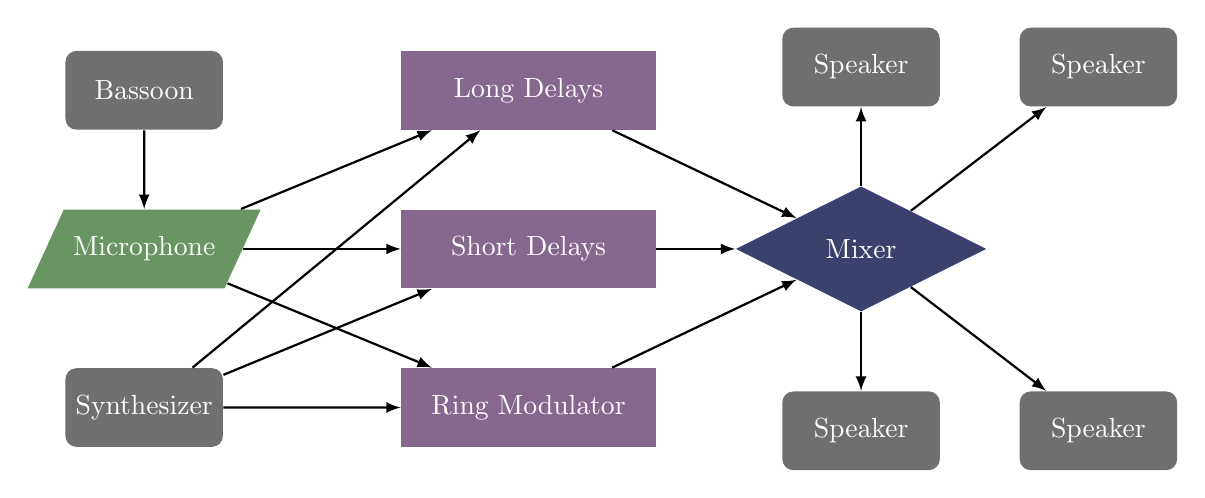
\begin{tikzpicture}[align=center, node distance=1cm]
  \node (bsn) [source] {Bassoon};
  \node (mic) [input, below = of bsn] {Microphone};
  \node (synth) [source, below= of mic] {Synthesizer};
  \node (verb) [processor, right= of mic, xshift=1cm] {Short Delays};
  \node (rmod) [processor, below= of verb] {Ring Modulator};
  \node (pitch) [processor, above= of verb] {Long Delays};
  \node (mixer) [routing, right= of verb] {Mixer};
  \node (speaker1) [source, above= of mixer] {Speaker};
  \node (speaker2) [source, below= of mixer] {Speaker};
  \node (speaker3) [source, right= of speaker1] {Speaker};
  \node (speaker4) [source, right= of speaker2] {Speaker};
  \draw [cable] (bsn) -- (mic);
  \draw [cable] (mic) -- (verb);
  \draw [cable] (mic) -- (rmod);
  \draw [cable] (mic) -- (pitch);
  \draw [cable] (synth) -- (verb);
  \draw [cable] (synth) -- (rmod);
  \draw [cable] (synth) -- (pitch);
  \draw [cable] (rmod) -- (mixer);
  \draw [cable] (verb) -- (mixer);
  \draw [cable] (pitch) -- (mixer);
  \draw [cable] (mixer) -- (speaker1);
  \draw [cable] (mixer) -- (speaker2);
  \draw [cable] (mixer) -- (speaker3);
  \draw [cable] (mixer) -- (speaker4);
\end{tikzpicture}

\end{document}
